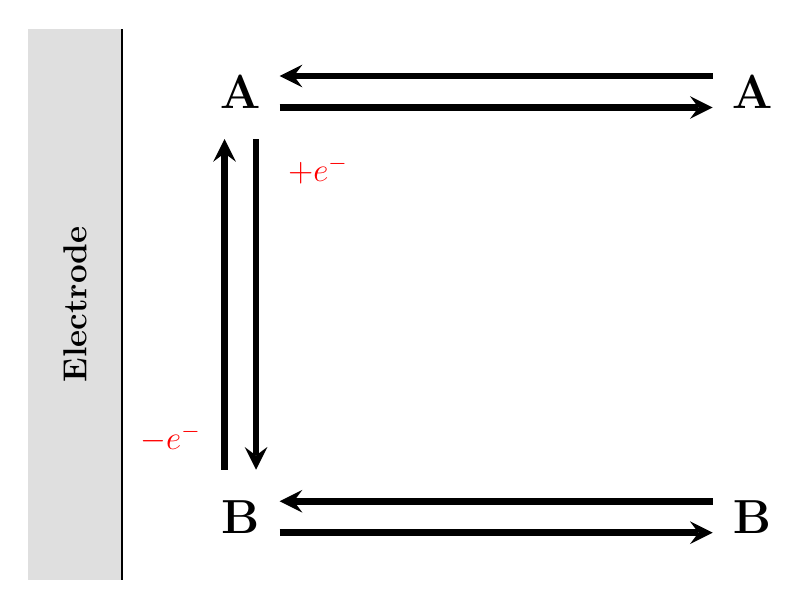
\begin{tikzpicture}[>=stealth, thick]

  % Electrode block
  \fill[gray!25] (-1.2, -1) rectangle (0, 6);
  \draw[thick] (0, -1) -- (0, 6);
  \node[rotate=90, font=\large\bfseries] at (-0.6, 2.5) {Electrode};

  % Species A row (top)
  \node[font=\LARGE\bfseries] at (1.5, 5.2) {A};
  \node[font=\LARGE\bfseries] at (8.0, 5.2) {A};
  % A: thick arrow from bulk towards electrode
  \draw[->, line width=2.5pt] (7.5, 5.4) -- (2, 5.4);
  % A: thin arrow from electrode towards bulk
  \draw[->, line width=2.5pt] (2, 5.0) -- (7.5, 5.0);

  % Species B row (bottom)
  \node[font=\LARGE\bfseries] at (1.5, -0.2) {B};
  \node[font=\LARGE\bfseries] at (8.0, -0.2) {B};
  % B: thin arrow from bulk towards electrode
  \draw[->, line width=2.5pt] (7.5, 0.0) -- (2.0, 0.0);
  % B: thick arrow from electrode towards bulk
  \draw[->, line width=2.5pt] (2.0, -0.4) -- (7.5, -0.4);

  % Electron transfer arrows (to the right of the electrode surface)
  \draw[->, line width=2.5pt] (1.7, 4.6) -- (1.7, 0.4);
  \node[right, font=\large] at (0.1, 0.8) {\textcolor{red}{$-e^-$}};

  \draw[->, line width=2.5pt] (1.3, 0.4) -- (1.3, 4.6);
  \node[left, font=\large] at (3.0, 4.2) {\textcolor{red}{$+e^-$}};

\end{tikzpicture}
